\documentclass[letterpaper,10pt,oneside,conference,final]{sbrt2015}
 
%\usepackage[utf8]{inputenc}
%\usepackage{graphicx}
\usepackage{enumerate}

\begin{document}
  \IEEEoverridecommandlockouts

  \title{On the stability of multiple delay-centric multi-homed transmissions}
  \author
  {
    \authorblockN{Pedro Mantovani Antunes, Guilherme de Souza Miguel,\\
                  Carlos M. Pedroso, Eduardo Parente Ribeiro\\}
    \authorblockA{Universidade Federal do Parana - UFPR\\
                  P.O. Box 19011 -- 81531-980\\
                  Curitiba -- PR -- Brazil\\
                  edu@ufpr.br}
%Instituto Nacional de Telecomunica��es - Inatel\\
%                  P.O. Box 05 - 37540-000 \\
%                  Santa Rita do Sapuca� - MG - Brazil\\
%                  ynoguti@inatel.br}
%    \and
%    \authorblockN{Jos� Marcos C�mara Brito}
%    \authorblockA{Instituto Nacional de Telecomunica��es - Inatel\\
%                  P.O. Box 05 - 37540-000 \\
%                  Santa Rita do Sapuca� - MG - Brazil\\
%                  brito@inatel.br}
  }
  \maketitle

  \begin{abstract}
    The use of multiple network access interfaces for multimedia transmission can reduce packet delay by choosing the less congested end-to-end path for transmission. Delay-centric is a simple mechanism that selects the path with current lowest delay. When many users employ this mechanism there is a possibility of instabilities due to excessive path changes that increases overall packet delay. In this paper we investigate some modifications on the delay-centric algorithm that are able to reduce overall transmission latency in a scenario with multiple independent transmissions.
  \end{abstract}

  \begin{keywords}
    multi-home, end-to-end multipath, delay-centric.
  \end{keywords}


  \section{Introduction}

  The multi-homing feature has been gaining increasing popularity in the recent years. Users can be connected to the Internet by different access technologies such as ADSL (Asymetric Digital Subscriber Line), Wi-Fi, Wimax (Worldwide Interoperability for Microwave Access), 3G and LTE (Long Term Evolution). Multimedia communication can benefit from multiple end-to-end paths by selecting the best available path for transmission at a particular time, thus avoiding congestion and reducing packet loss.

A framework for multi-homed communication was established by the Stream Control Transmission Protocol (SCTP) \cite{Stewart2007a}, but other approaches are possible, such as Multipath Transmission Control Protocol (MPTCP) \cite{Ford2013}\cite{Zekri2012}. The standard SCTP protocol monitors the availability of each end-to-end path and automatically switches transmission to a secondary path in case of failure in the primary path to increase resilience. Other utilizations of the multi-homing feature already proposed in the literature includes concurrent multipath transfer (CMT) \cite{Casetti2004}\cite{Ye2004}\cite{Iyengar2006}, seamless handoff for mobile users \cite{Koh2004}\cite{Ma2004} and delay-centric transmission for low-delay communication \cite{Kelly2004}\cite{Kashihara2004}. The latter is suitable for real-time multimedia transmissions.
The benefits of the delay-centric algorithm for a single multimedia transmission have already been shown by several authors \cite{Noonan2004b}\cite{Fitzpatrick2007}\cite{Gavriloff2009a}\cite{Runcos2010}. 

One topic that has not been fully investigated is the stability issue that arises when many users employ the same delay-centric mechanism to transmit over the available paths. An initial investigation has shown that under high link utilization, overall packet delay can increase due to excess of path changes of the transmitting sources \cite{Gavriloff2009}.
In this paper, we investigate some measures that can be taken to mitigate these instabilities and provide lower packet delays for all transmissions.

The remainder of this paper is divided into four sections. Section II describes some fundamentals of delay-centric SCTP transmission. Section III explains the implemented methods. Results are shown in Section IV e conclusion is presented in Section V.  

  \section{Multi-homed low delay communication}
  
  \subsection{Latency Estimation}

  Amongst other reasons, a latency estimation is necessary in both SCTP and TCP to calculate the retransmission timeout (RTO) of each packet. To achieve this estimation, these protocols compute the round trip time (RTT) of a packet every time an acknowledge is received. As this value is highly variable, the protocol also computes the smoothed round trip time (SRTT) as 
  \begin{equation}
   SRTT_i  = (1 - \alpha) SRTT_{i-1} + \alpha  RTT \\
  \end{equation}

  where $\alpha$ value is 0.125, as recommended by RFC 6298 \cite{Paxson2011a}.


  \subsection{Delay-centric}

  Delay-centric method compares the SRTT of all paths to decide where to transmit the packets \cite{Kelly2004}. The SRTT of the primary path is updated frequently, because it is changed every time a packet is transmitted and its ACK is received. In the secondary paths, the SRTT is updated only after a heartbeat (HB) is sent and a heartbeat-ack (HB-ACK) is received. This does not give these paths a proper estimation of the SRTT, as the standard interval value between HBs is 30\,s. To improve the algorithm's responsiveness, most authors employed the value of 1\,s for the HB interval \cite{Noonan2004b}\cite{Gavriloff2009}\cite{Torres2014}.

The path switches in delay-centric can occur when the difference of the SRTT of the current path and the SRTT of an alternate path becomes greater than zero, or greater than a threshold. This threshold in milliseconds is simply called hysteresis.

A variation of the pure delay-centric method is the setting of a guard-time \cite{Gavriloff2009a}. This is the period, in milliseconds, to wait after the SRTT comparison indicated a switchover. At the end of this period, the SRTTs are compared again, to check if the current SRTT is still greater than the SRTT of the alternate path, to confirm the switchover or to cancel it, and keep the transmission in the same path. We propose the use of a random guard-time instead of a fixed guard-time. The idea is avoid a synchronous operation of the sources and to promote better distribution of the decision instant over the time. We also propose the reduction in the heartbeat interval to 20\,ms during guard-time, in order to improve the estimative of the SRTT of the alternate path.

  \subsection{Predictive delay-centric}

  A recent improvement in the delay-centric method also considers the SRTT trend \cite{Torres2014}. The Moving average convergence divergence (MACD) method is used. For each path, two SRTTs are calculated. A short time version, with $\alpha = 0.667$, named $SRTT_S$, and a long time version, with $\alpha = 0.154$, named $SRTT_L$. When the $SRTT_S$ becomes greater than $SRTT_L$, there is a trend to increase latency. The proposed switchover algorithm takes this trend into account and performs the switchover only when these three conditions hold:
\begin{enumerate}[i)]
 \item $SRTT_S$ current path greater than $SRTT_S$ alternate path.
 \item Current path SRTT is increasing ($SRTT_S > SRTT_L$).
 \item $SRTT_S$ of current path is greater than a threshold, set at 150\,ms.
\end{enumerate}

Simulations with typical delays gathered from Wi-Fi, 3G and Ethernet, have shown that this strategy, called predictive delay-centric, improves the quality of video transmission and reduces the number of path switchovers compared to pure delay-centric, which is a reactive method.

In this paper, we propose a small alteration for better performance. We replaced condition (ii) of the algorithm by: ``The trend of increasing latency is greater in the current path than it is in the alternate path''. This alteration makes the protocol calculate the trends of the SRTTs of both primary and secondary paths, computing the difference between them. Switchover only occurs if the alternate path has a better tendency to reduce the latency than the primary path, and if conditions (i) and (iii) are also true. The modified method was used all along this paper, however both methods were tested and presented at the end of Results section, in order to provide proper comparison.

\section{Methods}

The test bed consisted of two computers connected to each other by two Ethernet links, as illustrated in Figure~\ref{topology}. Although the results can be extended to a greater number of paths, only two paths were considered in the tests. This number of two was chosen because of the simplicity for early simulations and because not many hardwares nowadays are found with more than two different links to the Internet.

\begin{figure}[h!]
\centering
%\includegraphics[width=8.5cm]{figuras/cadeiamark.ps}
%\includegraphics[scale=0.3]{gilbert}
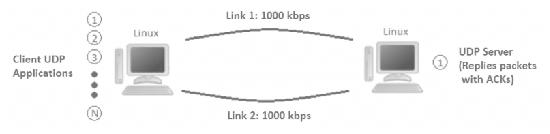
\includegraphics[width=8.5cm, height=2.2cm]{figura1}
\caption{Topology used in the experiments.}
\label{topology}
\end{figure}

Both machines operate with Linux operating system (distribution Debian 7.1, Linux kernel 3.2.63-2). Test programs were written in C and compiled with gcc version 4.7.2-5. The multimedia transmission data consisted of 6 sources that independently transmitted UDP packets with 250 bytes of size, including headers. Each source also transmits heartbeat packets of the same size in the alternate path. Heartbeat transmission interval was randomly chosen between 0.5\,s and 1.5\,s, after each heartbeat. All ACK packets have 52 bytes. Each multimedia source starts its transmission at a random time, on the first second of the experiment. In order to work with lower bit rates, the bandwidth of the transmission was limited with the kernel traffic control (tc). 

A total of 3000 packets were sent on each experiment, which was repeated 200 times to estimate the mean packet delay, standard deviation and confidence intervals. In each experiment, the mean packet delay was measured in function of the link utilization $\rho$. Its definition was extended to consider this multipath scenario, according to 

\begin{equation}
 \rho = \frac{B}{C}
\end{equation}
where B is the total traffic bit rate, which is given by the number of sources times the individual bit rate plus background traffic. C is the total paths capacity, which is given by the number of paths times the individual capacities. In the experiments, the individual path capacities were kept at 1000 kbps, which gives C = 2000 kbps. In the simulations, $\rho$ was varied from 0.66 to 0.99. 

The following mechanisms were tested:
\begin{enumerate}[i)]
 \item Pure delay-centric, hysteresis = 10\,ms, HB interval = 0.5 -- 1.5\,s.
 \item Delay-centric, hysteresis = 10\,ms, HB interval = 0.5 -- 1.5\,s (decreased to 20\,ms during guard-time), guard-time = 1 -- 4\,s. 
 \item Predictive delay-centric, HB interval = 0.5 -- 1.5\,s.
 \item Predictive delay-centric, HB interval = 0.5 -- 1.5\,s (decreased to 20\,ms during guard-time), guard-time = 1 -- 4\,s.
\end{enumerate}

Because the bandwidth was limited only in the sender machine, every queue delay was originated in the sender side as well. This doesn't reflect the actual Internet scenario, in which queue delays are originated in both ways of the links. To compensate this problem caused by our topology, we changed the switchover threshold in the predictive delay-centric experiments to 70\,ms.

The mechanisms number (i) and (iv) were also simulated with the presence of background traffic. The background traffic consisted of fixed size UDP packets (250 bytes) with random, exponentially distributed inter-arrival time. Different proportions of background and foreground traffic were analyzed, but in order to simplify the results, we decided to present only the proportion of 40\% background traffic against 60\% of foreground traffic, which gives a representative comparison between both mechanisms in a different scenario.

\section{Results}
\subsection{Algotihms' Behavior}
  A first round of experiments was performed without background traffic. For low utilization ($\rho < 0.75$) the distributed delay-centric mechanism was able to promote an even distribution of the transmissions over the two paths. For higher utilization ($\rho > 0.75$), instabilities occur and the excessive path changes increase the overall mean delay. 

For a particular high utilization, after 200 transmissions, the mean delay for each transmission was recorded. The observed histogram does not have a single mode, but have two modes. One mode is close to zero (minimum delay) and the other mode is between zero and the maximum delay. The interpretation of this result is that with some initial conditions, delay-centric mechanism was able to correctly distribute all flows on the available paths and achieve low mean delay for all flows. But other initial conditions led to non-stable behavior and delay-centric kept changing paths resulting in large mean delays for all flows. Figure 2 displays the mean delay as a function of the utilization.

\begin{figure}[h!]
\centering
%\includegraphics[width=8.5cm]{figuras/cadeiamark.ps}
%\includegraphics[scale=0.3]{gilbert}
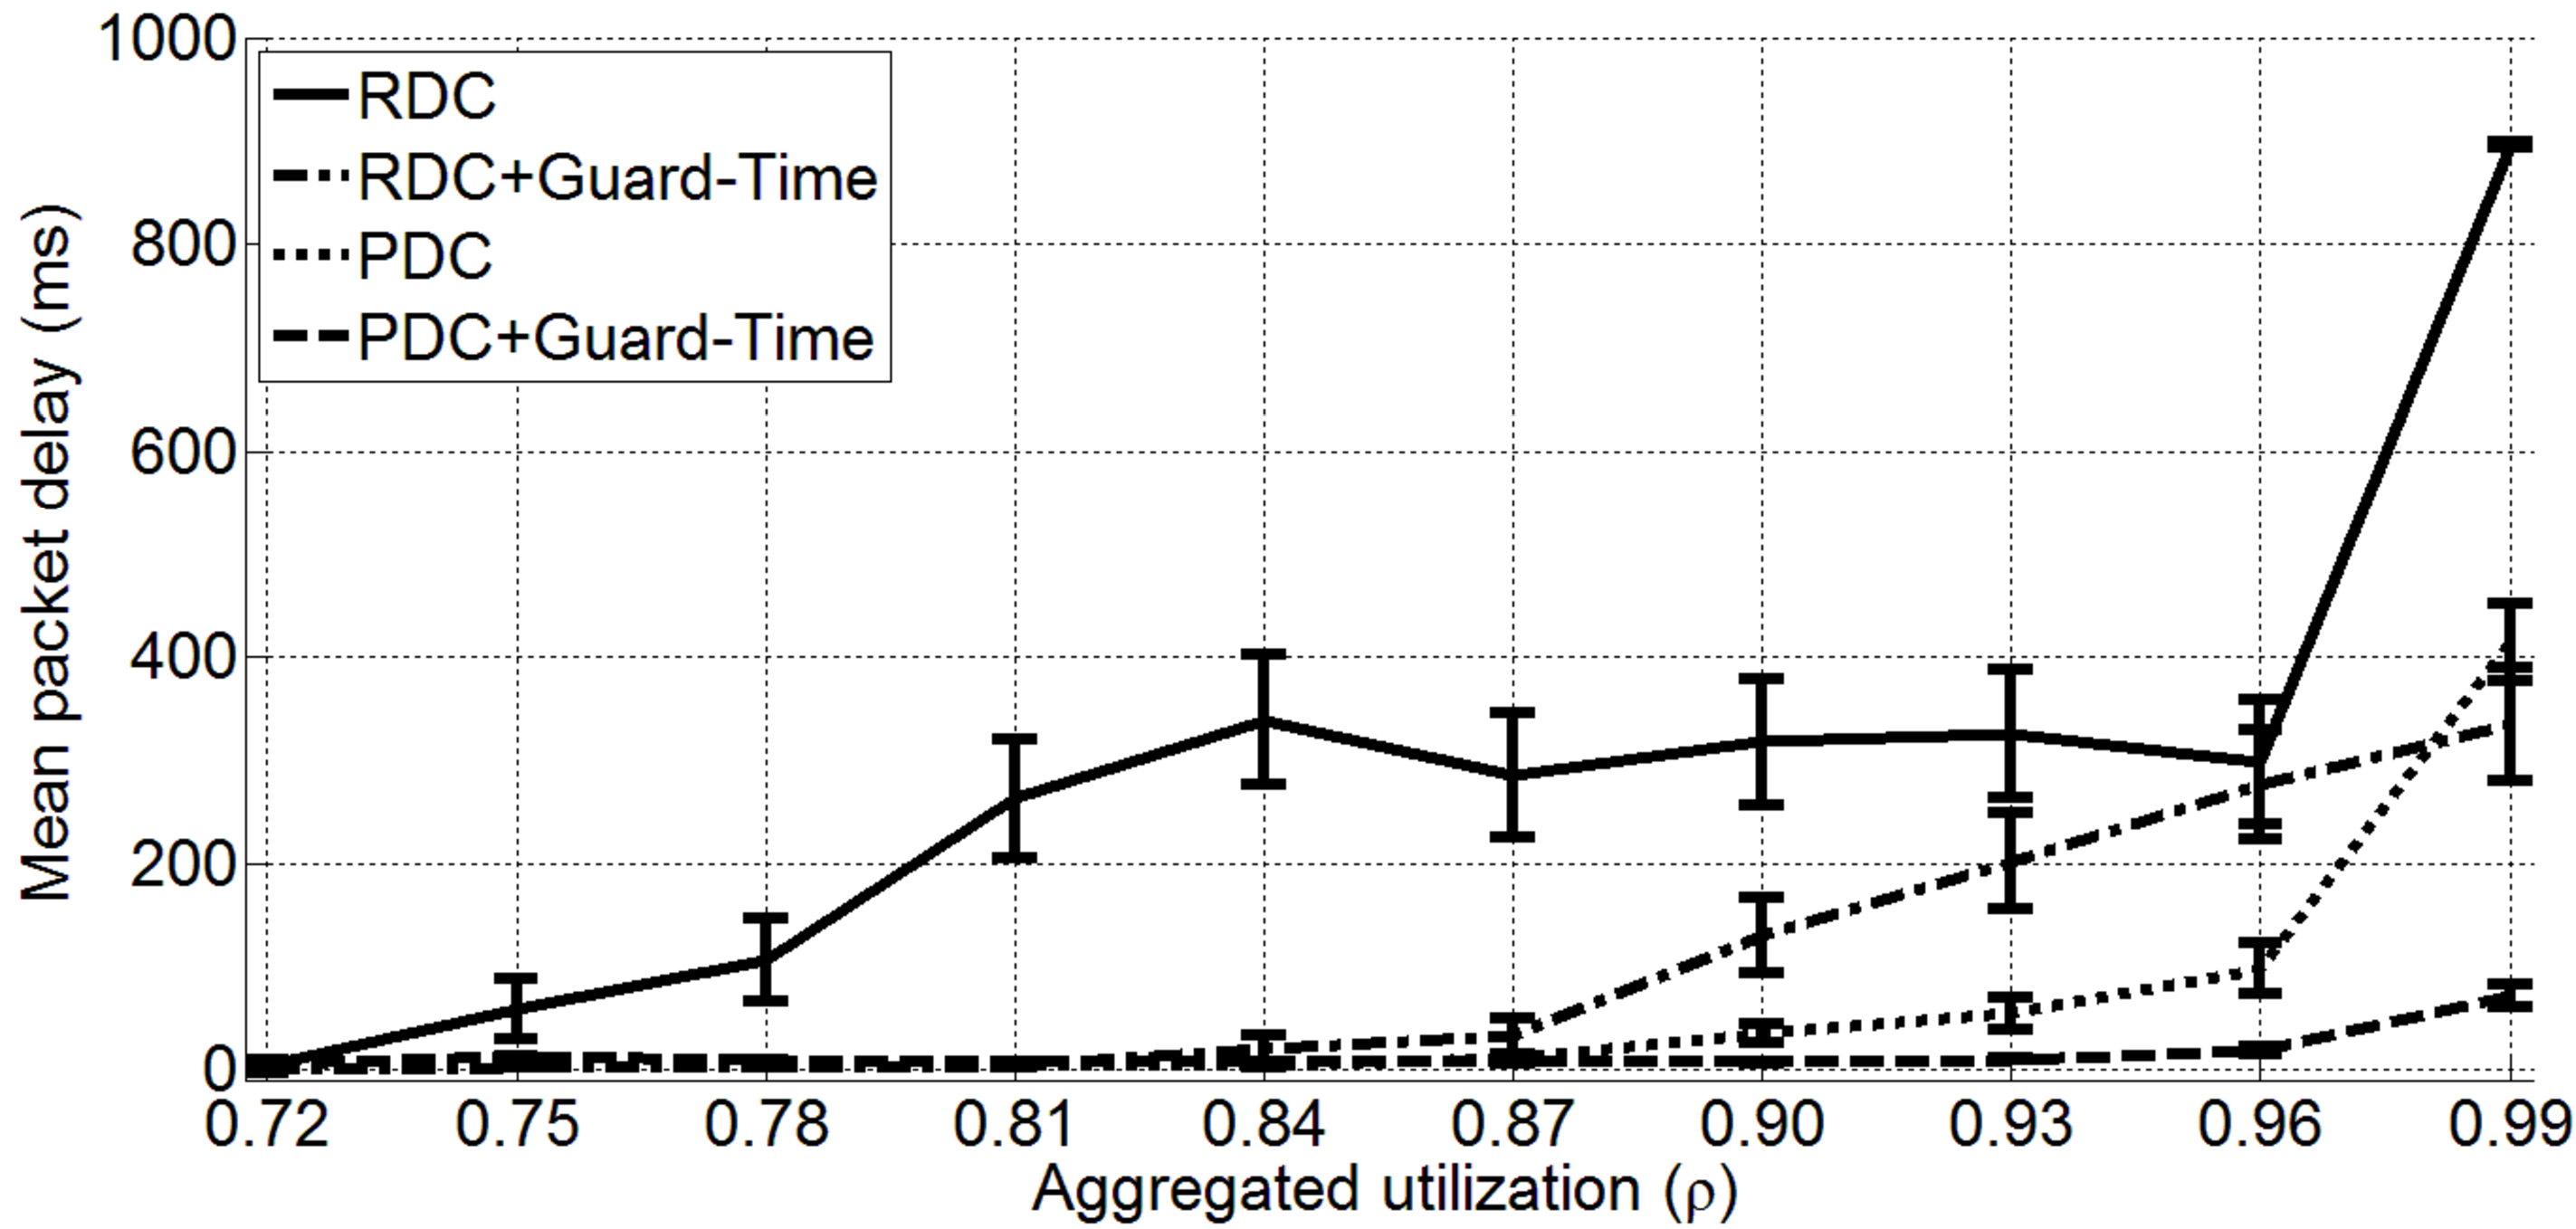
\includegraphics[width=8.8cm,height=4.5cm]{figura2}
\caption{Pure low delay-centric.}
\label{figura2}
\end{figure}

In Figure~\ref{figura2}, the dashed curve on the top is the higher mode, which represents cases of instabilities. The dotted curve in the bottom is the lower mode, which clearly stands for the cases of good stabilitiy, as the delay goes to almost 0\,ms. For each curve, confidence intervals (95\%) are plotted. 

The central curve is the overall mean packet delay, regardless of the mode. This is probably the most important information of the Figure, though the modes are also interesting information to check how the cases of stability and instability are distributed along the axes.

The next experiment, represented in Figure~\ref{figura3}, was executed with the guard-time allied to the delay-centric algorithm, with the reduction of the HB interval during guard-time, as explained in Section III. The two modes were still present in the experiment, which indicates the existence of instability in some cases.

\begin{figure}[h!]
	\centering
	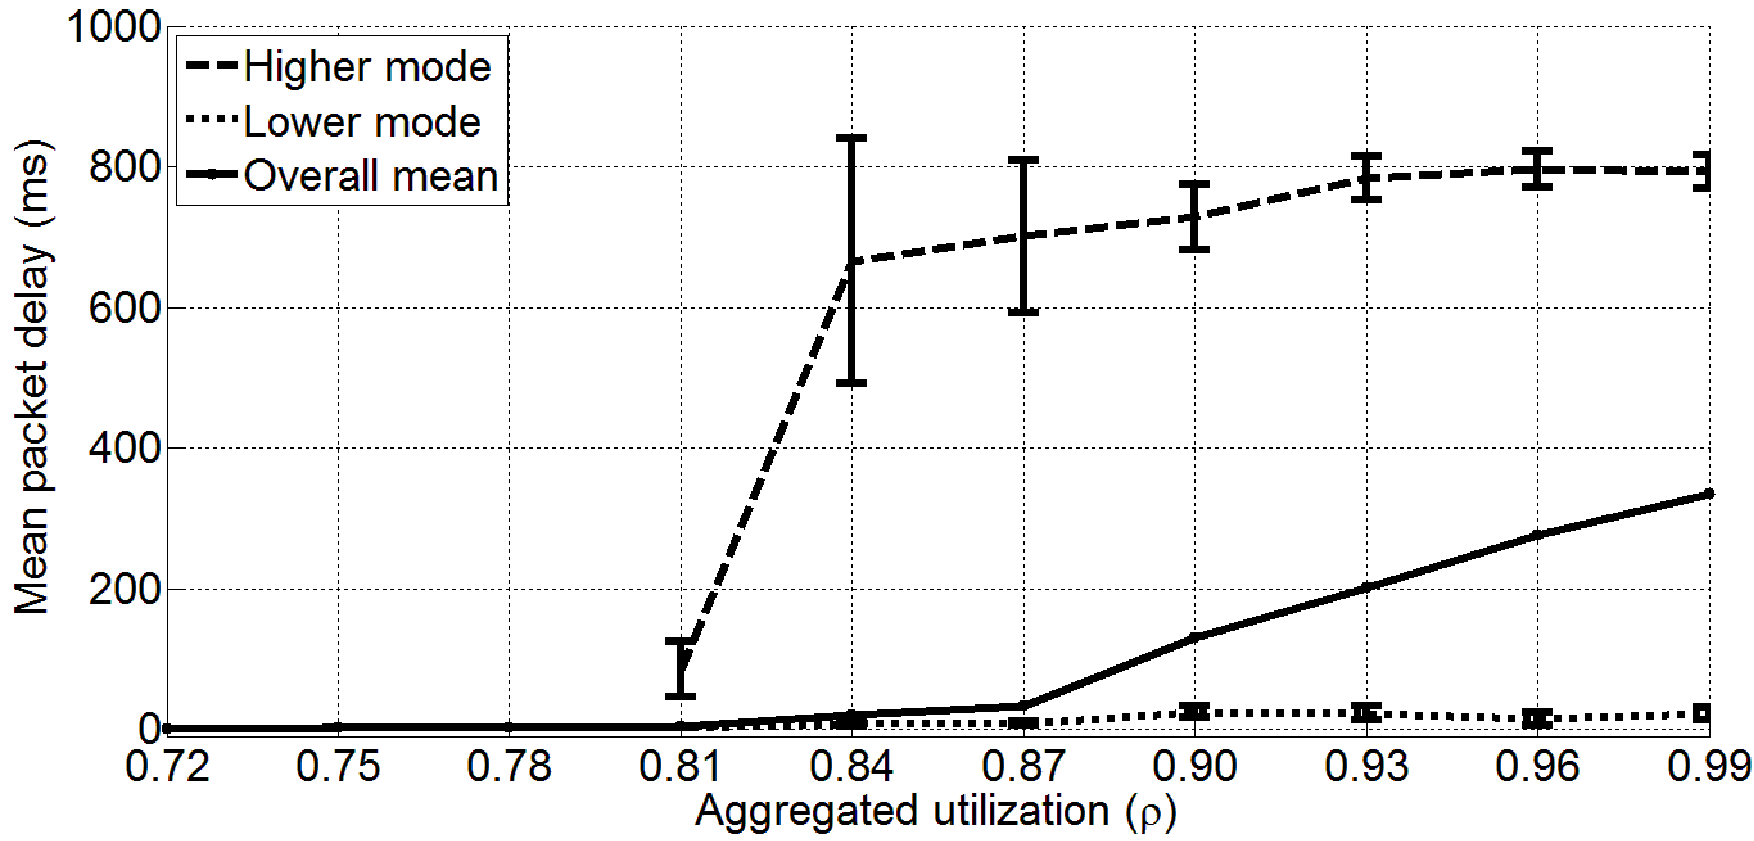
\includegraphics[width=8.8cm,height=4.5cm]{figura3}
	\caption{Guard-time with HB interval reduction.}
	\label{figura3}
\end{figure}

As can be noted in Figure~\ref{figura3}, this latter algorithm, compared to the pure delay-centric, had a great reduction of the overall delay of the packets, which may be due to the decrease of HB interval. This may have given the sources a better estimative of the SRTTs, leading to a better path decision. 

The predictive delay-centric was evaluated next. The MACD algorithm was tested twice: a simple predictive delay-centric, and a predictive delay-centric with guard-time and HB interval reduction. These experiments are represented respectively in Figure~\ref{figura4}, and Figure~\ref{figura5}.


\begin{figure}[h!]
\centering
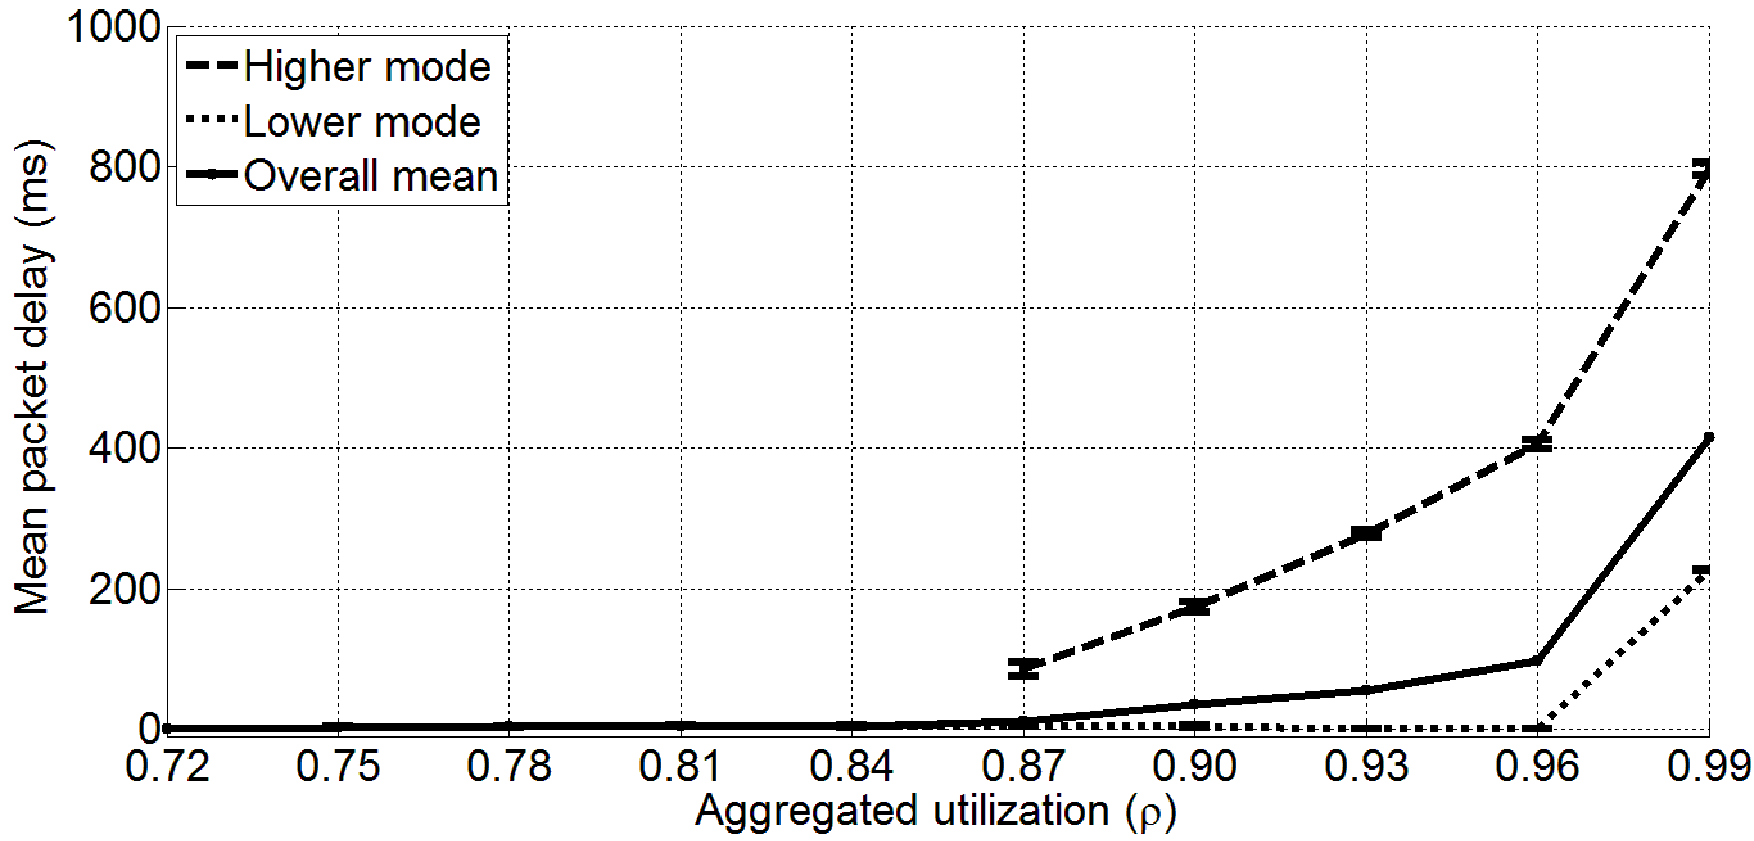
\includegraphics[width=8.8cm,height=4.5cm]{figura4}
\caption{Simple predictive delay-centric.}
\label{figura4}
\end{figure}


The pure MACD algorithm resulted in lower mean packet delay than the pure delay-centric, which indicates its natural trend to avoid instabilities. Even in cases of instability, it is noticed that in the predictive delay-centric the higher mode delay is lower than in the reactive delay-centric.

\begin{figure}[h!]
\centering
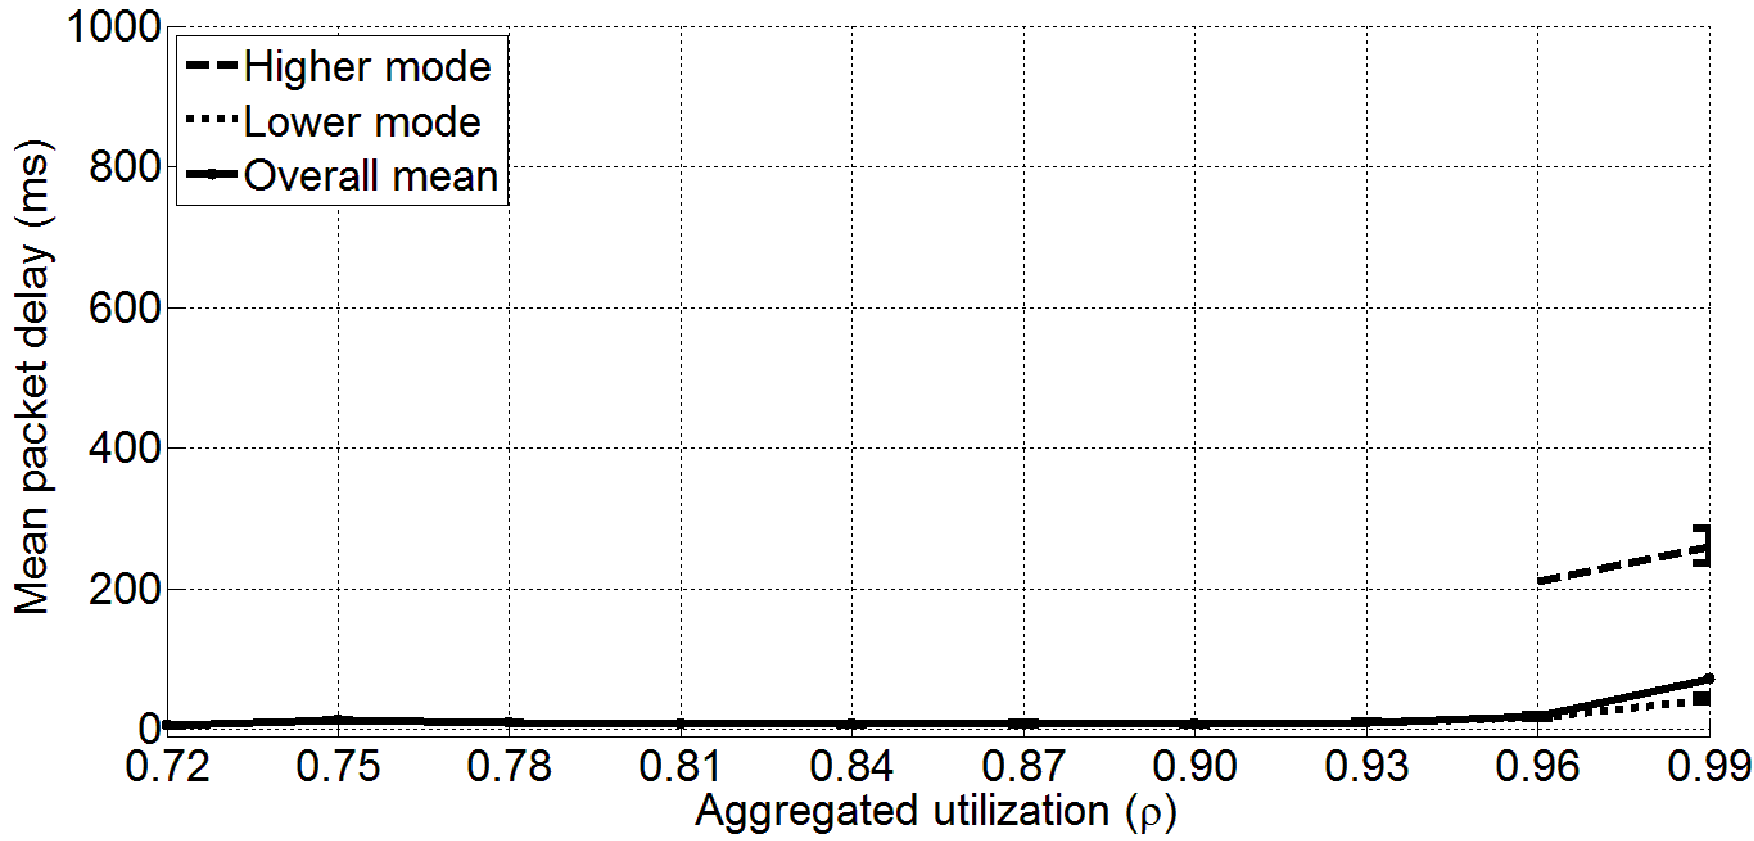
\includegraphics[width=8.8cm,height=4.5cm]{figura5}
\caption{Predictive delay-centric with guard-time and HB interval reduction.}
\label{figura5}
\end{figure}

Following the tendency from the delay-centric, the guard-time implemented in predictive delay-centric helped even more to lower the overall mean packet delay, eliminating almost every case of instability. With this algorithm, even in the highest utilizations, the overall delay is not high enough to greatly affect the QoS of a VoIP call, for example.

\subsection{Background Traffic Scenario}
Afterwards, experiments were made with background traffic to investigate the superiority of the last mechanism (Figure~\ref{figura5})  in a different and more realistic scenario. In this situation, random delays were caused in the sending queue by the exponentially distributed interval between packet sends. We noted that the addition of background traffic improved the stability of the algorithms. Different and random transient delays may have helped unbiased path choice.

Figure~\ref{figura6} presents the comparative between all the previous tested methods, in which only the overall mean packet delay is showed. In this simulation, all the sources represent 60\% of the total traffic, while the exponential background traffic represents only 40\% of total traffic.

\begin{figure}[h!]
\centering
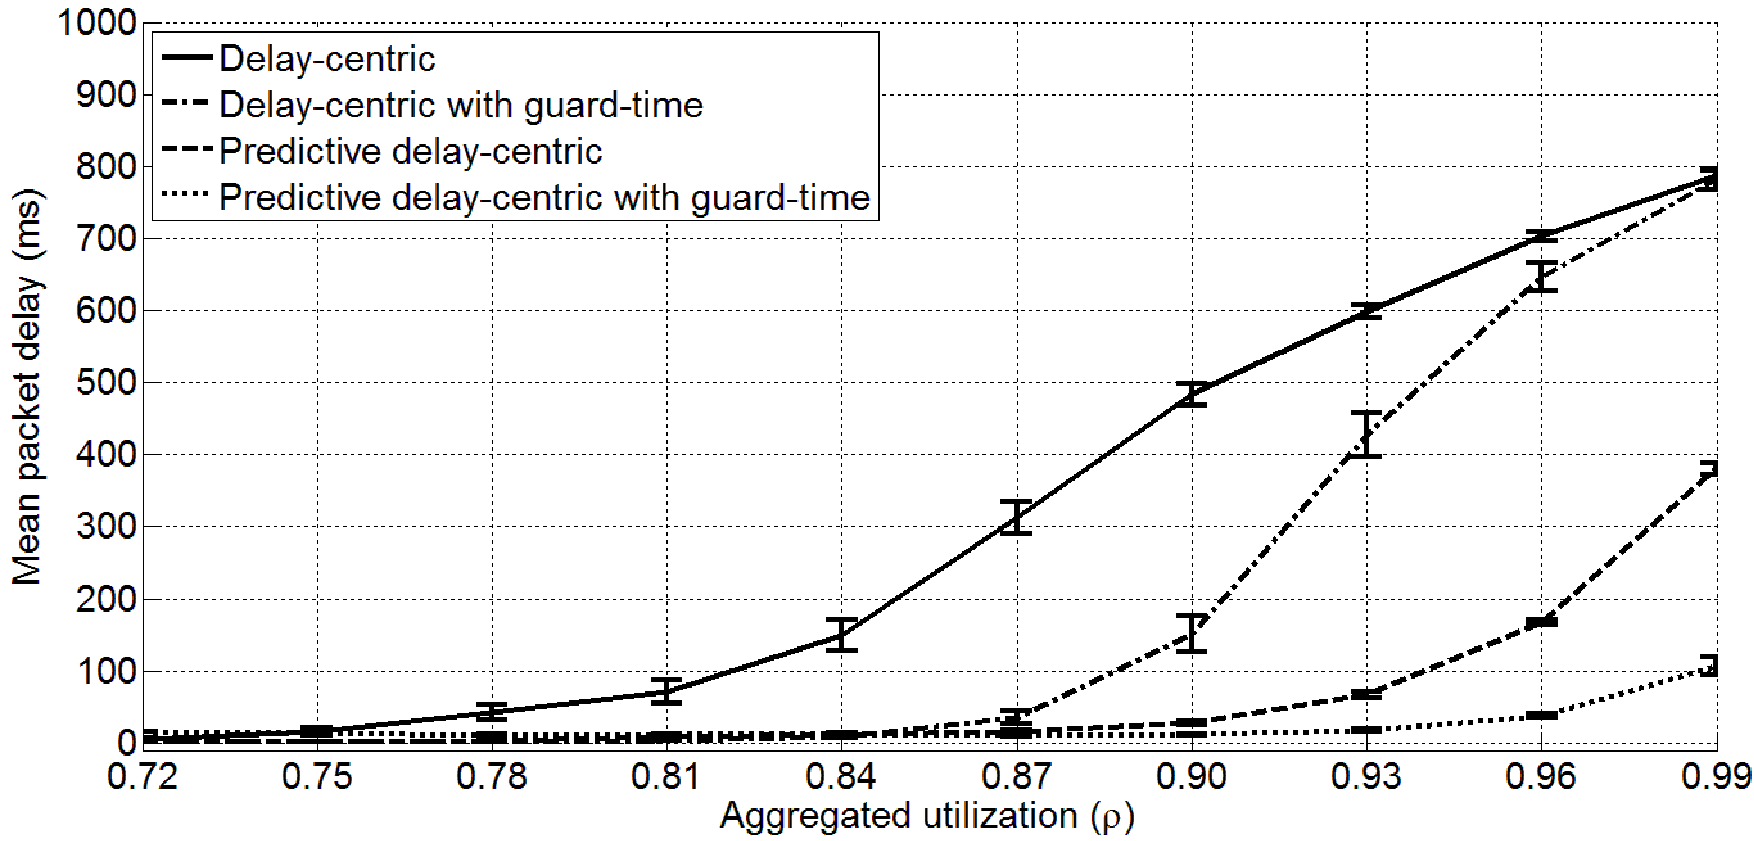
\includegraphics[width=8.8cm,height=4.3cm]{figura6}
\caption{Scenario with random background traffic.}
\label{figura6}
\end{figure}

Even in a more realistic scenario, with background traffic, it is visible in Figure~\ref{figura6} that the predictive delay-centric with guard-time had a much better response than all the other algorithms, keeping a low delay for all sources of transmission.

\subsection{Comparison of Predictive delay-centric methods}
As explained in section II, the predictive delay-centric method used so far was the algorithm that analyzes the latency trend of all paths. In the original method only the trend of the primary path is analyzed. In Figure~\ref{figura7}, a comparison is made between the original method and the modified method in a scenario with background traffic. Both algorithms were tested with and without the presence of the guard-time.
Without the guard-time, the algorithms acted almost in the same way, and the mean packet delay is almost equal. This is due to the low proportion of packets in the secondary path comparing to the primary. With the guard-time implemented, the modified method exhibited lower delays in the highest utilization levels. The trend of secondary paths could now be calculated more precisely because of the decrease in the HB interval during guard-time. This behavior assisted the algorithm to distribute the transmissions evenly among the paths.

\begin{figure}[h!]
	\centering
	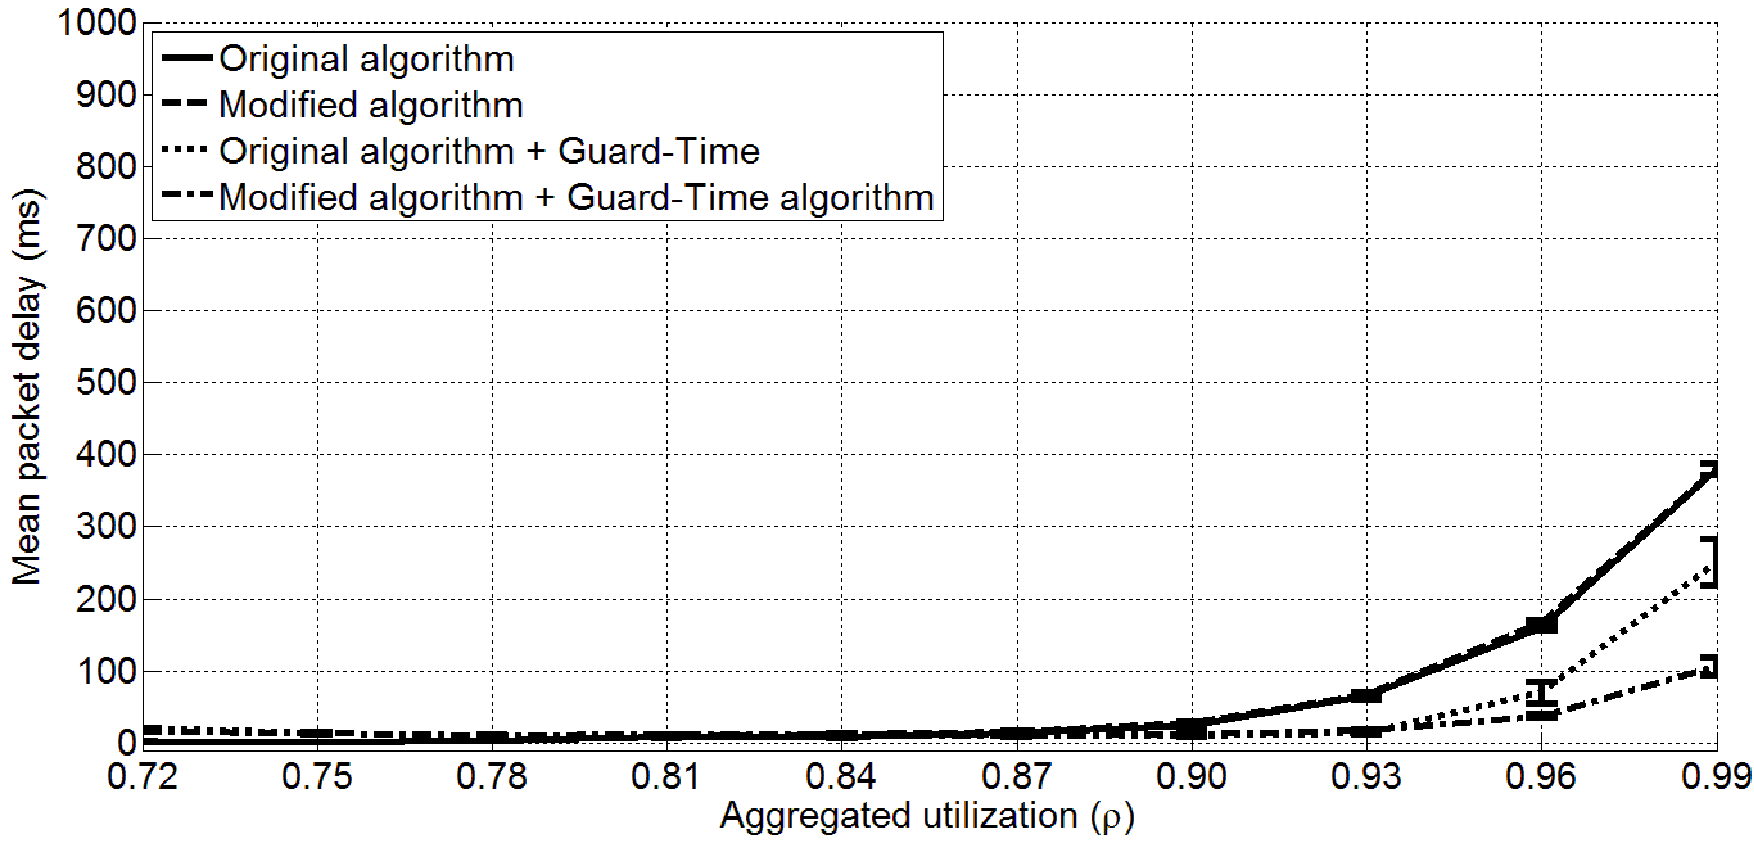
\includegraphics[width=8.8cm,height=4.3cm]{figura7}
	\caption{Comparison between predictive delay-centric methods.}
	\label{figura7}
\end{figure}

\section{Conclusion}

Low-delay communication is a desired condition for multimedia transmission, especially in real-time scenarios, such as VoIP calls and video streaming. Although delay-centric mechanism for multi-homed communication has been efficient to reduce packet delay by selecting the path with smaller SRTT, some instabilities may occur during high utilization, when many sources use the same mechanism. This could be a serious problem if the mechanism becomes standard in the SCTP protocol. We confirmed the existence of such instabilities in transmission between two computers with two interface cards.

One cause of instability is the poor sampling of actual smoothed round trip time of the alternate path. Modification of delay-centric with the introduction of a guard-time and frequent updates of the SRTT in the alternate path significantly reduced these instabilities and consequently the overall mean packet delay.

The predictive delay-centric, using trend comparison of current and alternate path also proved to be efficient in reducing the instabilities. The predictive delay-centric with guard-time and HB interval reduction proved to eliminate almost every instability in the switchover mechanism. A scenario with background traffic was also investigated, and once more the  transmission using predictive delay-centric and guard-time could be performed at higher utilization with lower latency in the sending of packets, comparing to the traditional delay-centric mechanism.


 %\begin{thebibliography}{2}
  %  \bibitem {Lamport} L. Lamport, \textit{A Document Preparation
  %  System: \LaTeX, User's Guide and Reference Manual}. Addison
  %  Wesley Publishing Company, 1986.
  %  \bibitem {Shell} M. Shell, ``How to use the IEEETran \LaTeX class'',
  % \textit{Journal of \LaTeX class files}, vol. 1, no. 8, pp.
  %  1-22. August 2002.
  %\end{thebibliography}

\bibliographystyle{IEEEtran}
\bibliography{referencias}

\end{document}
